\chapter{Project plan}
\label{cha:plan}

\section{Improving the debugging experience}

The plan for improving Gillian's debugger more or less follows on from the evaluation of the precious one~\cite{gillian-debugging-2021}.

\subsection{Building a custom debugging UI}

As stated in \autoref{sec:intro:debugging}, the DAP doesn't have the command
set necessary for debugging symbolic execution. We can, however, use a
combination of Webviews and custom DAP requests / events to supplement the
existing debugging UI (see \autoref{sec:background:extending-dap}).

\subsection{Selecting symbolic execution branches}

A prime missing feature as the debugger stands is the ability for users to
select branches of execution when debugging. Currently, the debugger runs
through the problem top-to-bottom, dealing with each branch in turn. Ideally,
users will able to select which branch to go down when given a choice.

\begin{figure}
  \noindent
  \makebox[\textwidth]{
    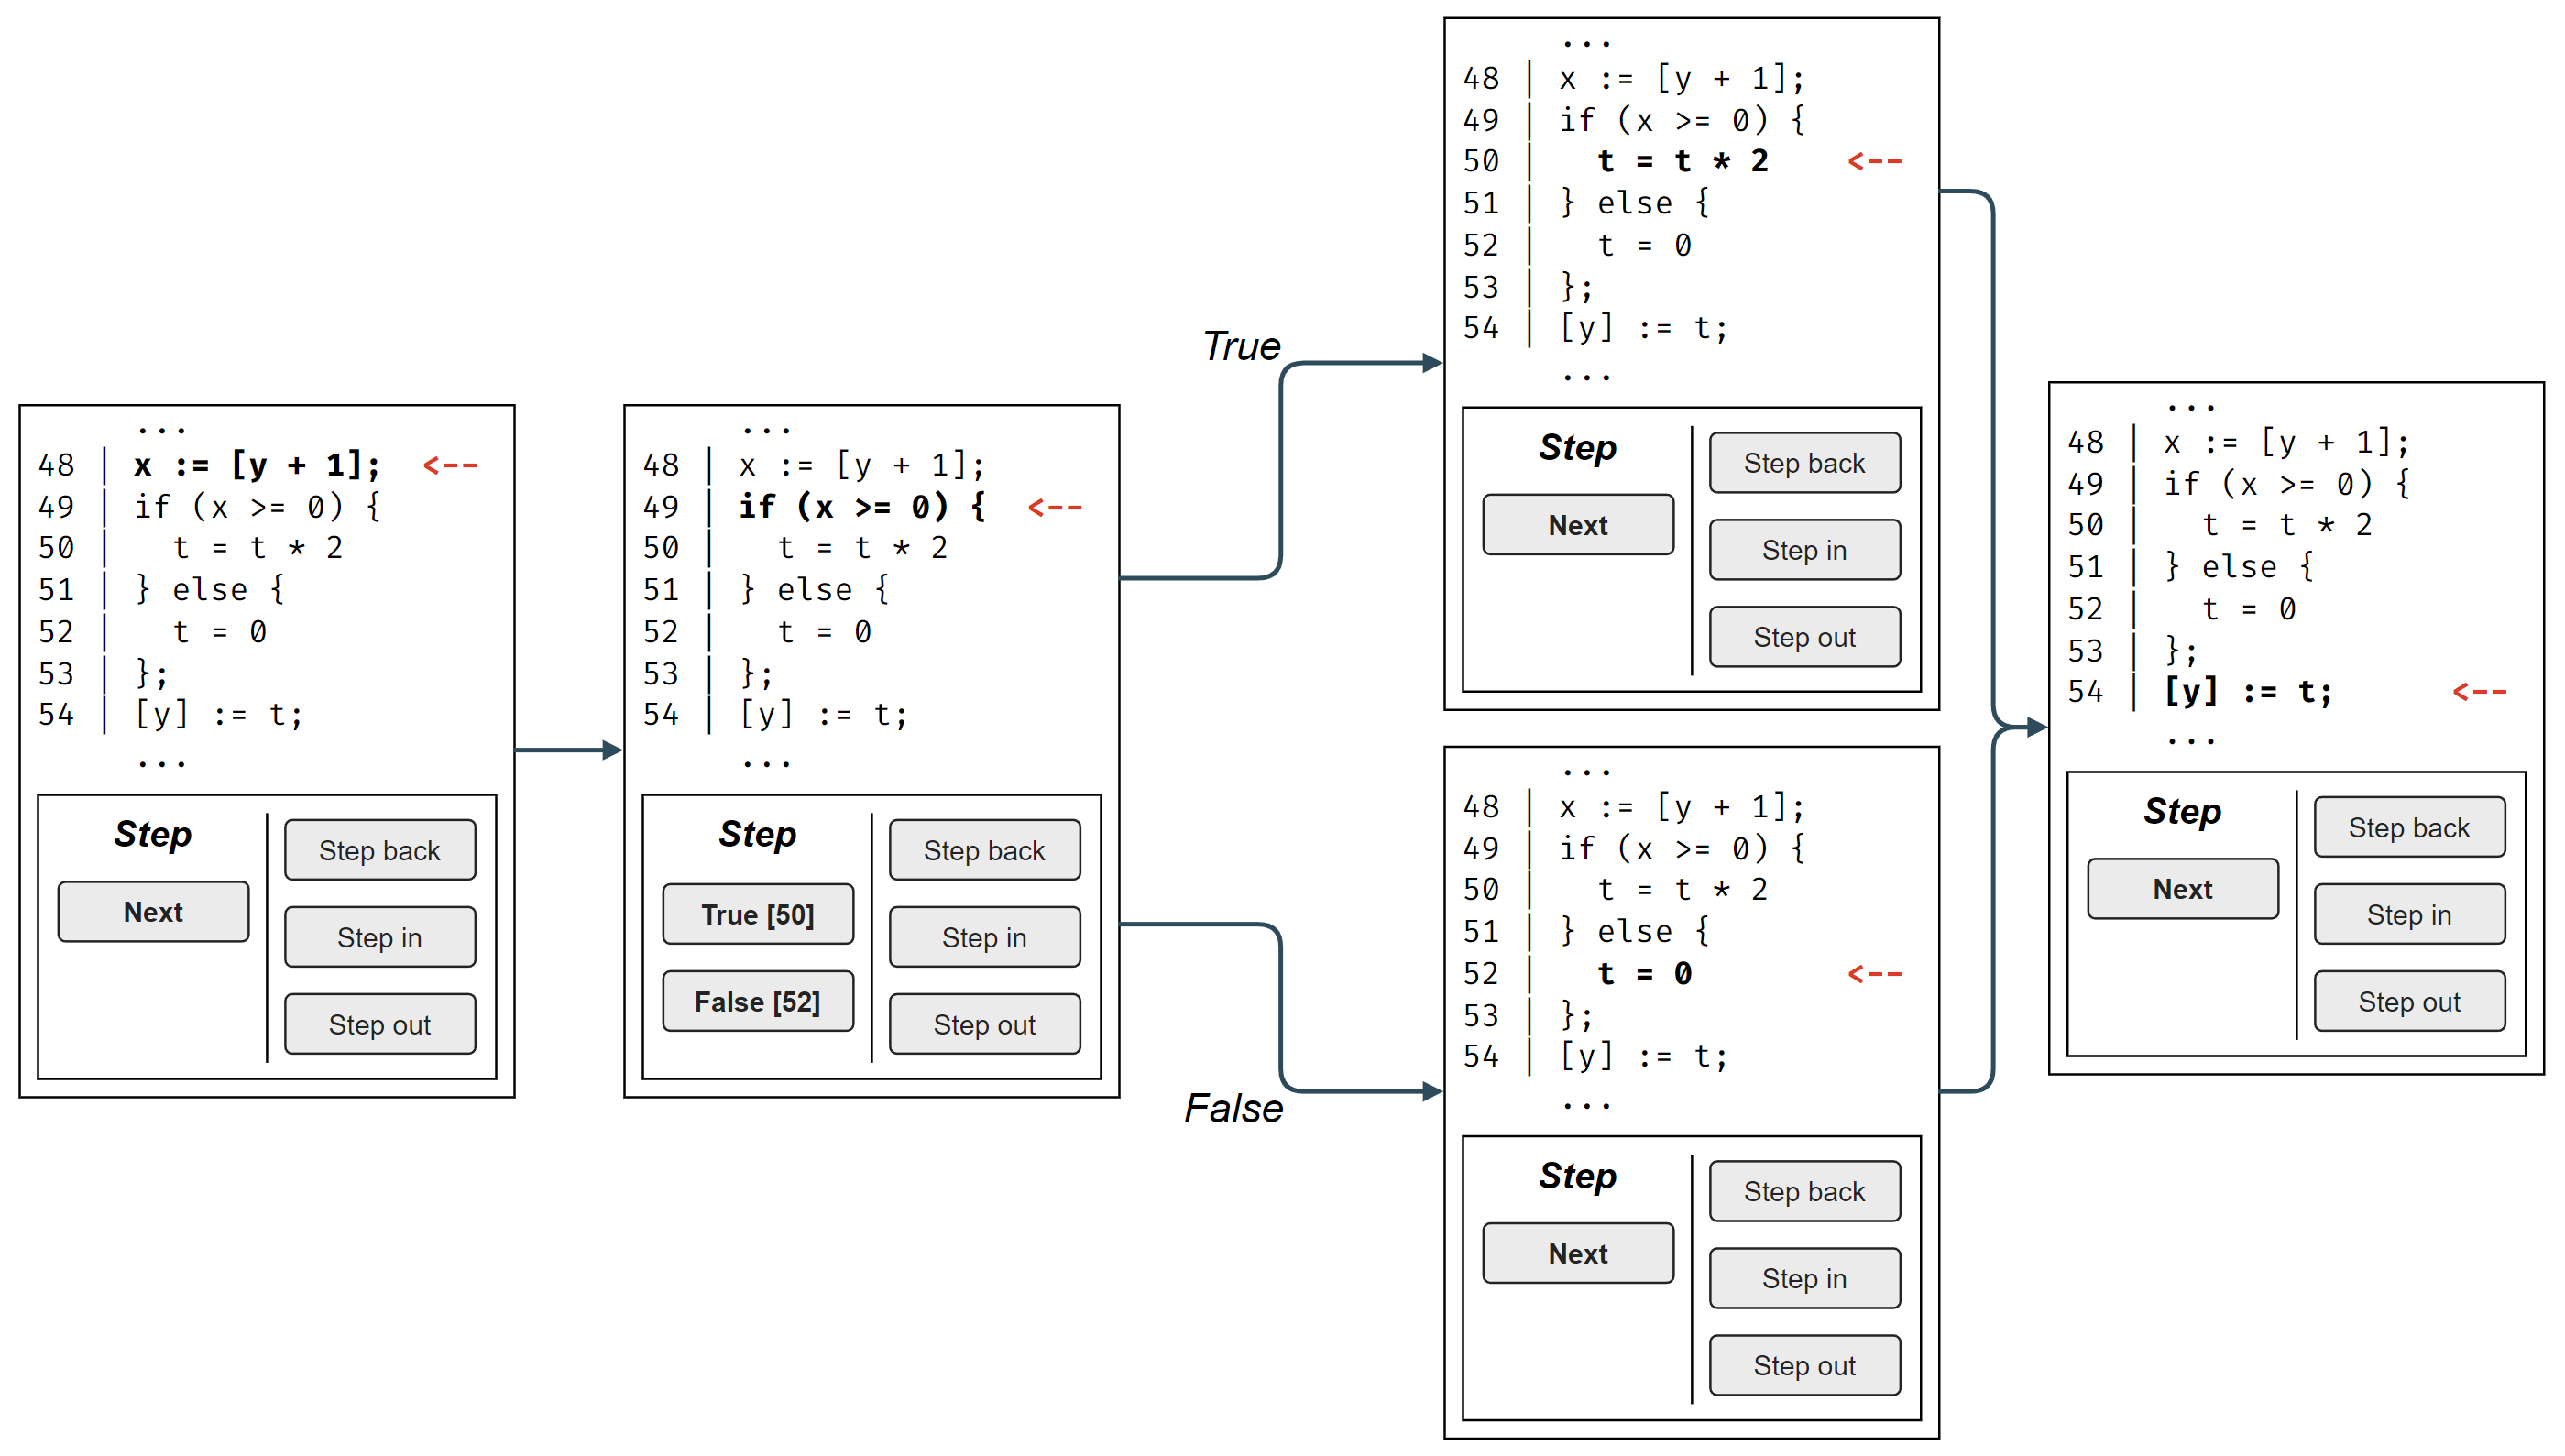
\includegraphics[width=500px]{img/branch-selection-mockup.png}
  }
  \caption{A mock-up of a potential UI flow for selecting execution branch.}
  \label{fig:branch-selection-mockup}
\end{figure}

As a bare minimum, this should be implemented for if-else statements; ideally,
this should be extended to cover switch statements, as well as any other
branching statements in the target languages supported.

% Maybe run an HTTP server when debugging to serve the extra info and controls?


\subsection{Improving error message coverage}

Whilst the Gillian debugger's coverage of error messages is mostly complete, it
is currently unable to give error messages for memory leaks, as debugging
unification is not supported. Rectifying this is one of the goals of this
project.

The debugger also does not yet support lifting JavaScript memory errors; this
should be achievable, as missing resource errors are the only form of memory
error for JavaScript.

As stated in the evaluation of the previous project, the debugger is entirely
focused on symbolic execution errors. To turn Gillian's debugger into a tool
that can be comfortably used by real developers, having the debugger encompass
more error types should be worked towards.


\subsection{Miscellaneous quality-of-life features}

There are a number of niceties that can be achieved in this project. A natural
extension of being able to select branches of execution is a full tree
visualisation of execution paths, allowing developers to jump forwards or
backwards (or 'sideways', in a sense) to any step of execution. Potentially,
small details such as showing resources that have been freed, à la VeriFast,
could be implemented; this purely depends on available time, and what would and
wouldn't be deemed useful by Gillian's primary developers and users.


\section{Gillian-Rust}
% What am I doing with Rust? Just implementing a debugger component for it?

A potential goal for this project is implementing Gillian debugging for the
Rust programming language~\cite{rust}. This is not a certainty, as it depends
both on how much time is available, and on the progress of another final year
project taking place in parallel with this one.
